% Created 2025-02-11 Tue 11:43
% Intended LaTeX compiler: xelatex
\documentclass[a4paper,12pt]{article}
\usepackage{graphicx}
\usepackage{longtable}
\usepackage{wrapfig}
\usepackage{rotating}
\usepackage[normalem]{ulem}
\usepackage{capt-of}
\usepackage{hyperref}
\usepackage{lmodern}
\usepackage{fontspec}
\usepackage[french]{babel}
\usepackage{amsfonts,amssymb,amsmath,mathrsfs,stmaryrd}
\usepackage[default]{sourcesanspro}
\usepackage[top=2.4cm, bottom=2.4cm, left=2.16cm, right=2.16cm]{geometry}
\usepackage{setspace,fancyhdr,indentfirst,adjustbox,caption,multicol,lastpage,datetime,authblk,ifthen}
\setlength{\columnsep}{0.8cm}
\usepackage[toc,page]{appendix}
\usepackage{array,booktabs,multirow,tabularx,colortbl,diagbox,makecell,ltablex}
\usepackage{enumitem}
\usepackage{graphicx,xcolor,pgf,tikz,pgfplots,pgfplotstable}
\usepackage[table]{xcolor}
\usepackage{algorithm2e,algorithm,arydshln,subcaption}
\usepackage{forest}
\usepackage[acronym]{glossaries}
\usepackage{fvextra,csquotes}
\usepackage{listings}
\usepackage{microtype}
\usepackage[colorinlistoftodos]{todonotes}
\usetikzlibrary{calc,positioning,shapes,arrows,arrows.meta,fit,automata,quotes}
\pgfplotsset{compat=1.18}
\makenoidxglossaries
\setcounter{page}{1}
\setlength{\marginparwidth}{1.6cm}
\setlength{\parindent}{0pt}
\setcounter{secnumdepth}{0}
\usepackage[colorinlistoftodos]{todonotes}
\usepackage{microtype}
\usepackage{orcidlink}
\usepackage{wrapfig}
\definecolor{wikipediablue}{HTML}{0645AD}
\let\cite\autocite
\hypersetup{colorlinks=true, linkcolor=wikipediablue, citecolor=wikipediablue, urlcolor=wikipediablue}
\usepackage{url,hyperref}
\end{multicols}
\author{Cyprien PIERRE \orcidlink{0009-0009-9040-6795}}
\date{2025-02-11}
\title{Méthode de sélection et de configuration des représentations graphiques des corpus d'informations}
\hypersetup{
 pdfauthor={Cyprien PIERRE \orcidlink{0009-0009-9040-6795}},
 pdftitle={Méthode de sélection et de configuration des représentations graphiques des corpus d'informations},
 pdfkeywords={},
 pdfsubject={},
 pdfcreator={Emacs 28.1 (Org mode 9.7.19)}, 
 pdflang={French}}
\usepackage[style=backend=biber,style=iso-numeric,doi=true,isbn=true,autocite=superscript]{biblatex}
\addbibresource{~/bib/references.bib}
\begin{document}

\maketitle
\begin{abstract}
Rédiger l'abstract ici
\end{abstract}

\renewcommand\{\keywordsname\{\textbf{Mots clés : }\keywords{Visualisation de données, Graphique, Méthode}

\begin{multicols}{2}
\section*{Introduction}
\label{sec:org5d56c7e}
La visualization de donnée est une discipline ancienne à la littérature riche et précise. Cependant, il n'existe, à ce jour pas de synthèse opérationnelle ni de méthode harmonisée dans la conception des représentations graphiques des informations. Ce rapport vise à fournir un point de départ cohérent à de futurs travaux en représentation visuelle d'informations. Il est basé sur une revue de littérature rigoureuse et les recommendations qu'il porte sont issues des lectures réalisées. Une tentative est réalisée d'objectiver les usages des diverses représentations.

L'origine de ces travaux prend place dans un besoin grandissant de solution de visualization d'information dans le secteur de la construction. Les technologies de Big Data, BIM, VDC et les disciplines de la science des données ont fortement pénétré ce secteur sur l'ensemble du cycle de vie des ouvrages. \autocite{asiauniversitytaichungtaiwanResearchApplicationFunctiontechnologyaesthetics2020} L'utilisation renforcée de l'IoT, l'émèrgence des BIS et BOS et l'intégration des solutions d'intelligences artificielles renforcent d'autant plus la nécessité pour ce secteur de se doter de moyens robuste en exploration et en communication des informations.

Le secteur de la construction est historiquement peu digitalisé en comparaison avec les autres industries. Pour adresser ce retard, il est important de publier des études opérationnelle claires et industrialisables dont chaque acteur de l'industrie de la construction puisse bénéficier immédiatement. Ce rapport s'inscrit dans cette démarche.

Il existe de multiples manières d'interargir avec un graphique. \autocite{schwabishCenteringAccessibilityData2022a,frankelavskyRightToolsJob2022}

Ce rapport aborde les éléments impliquant la mise en oeuvre de solution programmatique d'accessibilité et pouvant intégrer une logique globale de préparation de graphiques numériques tels que:
\begin{itemize}
\item L'exploration visuelle
\item La lecture des tables
\item L'écoute des descriptions
\item La sonification des données
\item L'interractivité avec les commandes de clavier
\end{itemize}

Ce rapport n'aborde pas les éléments nécessitant l'emploi de matériels spécifiques tels que :
\begin{itemize}
\item L'exploration en réalité mixte
\item Les retours haptiques
\item L'emploi d'écran à relief (braille)
\end{itemize}
\section*{Démarche}
\label{sec:orgd39b125}
La conduite de cette revue s'est déroulé de la manière suivante :
Nous avons commencé par dresser un panorama des types de graphiques existant en nous appuyant sur les travaux de \og From Data to Viz\fg{} \autocite{yanholtzDataViz2018}, \og The Graphic Continuum\fg{} \autocite{jonathanschwabishGraphicContinuum2014}, \og Lexique Visuel\fg{} \autocite{alansmithLexiqueVisuel}, \og Insights for ArcGis\fg{} \autocite{lindabealeInsightsArcGIS2017}.
Cette première action nous a permis de pré-catégoriser les graphiques selon leurs utilisation.

Ensuite, nous avons étudié les livres de divers auteurs et en avons tirés un ensemble de rêgles générales quant à la préparation des graphiques. Cela concerne les aspects visuels (couleurs, polices\ldots{}), des conseils sur la pertinence dans le choix des types graphiques suivant les objectifs attendus, quelques éléments d'accessibilités et des retours d'expériences. Sur cette base, nous avons affiné la catégorisation préétablies et commencé à regrouper les recommendations.

Pour compléter les dispositions propres à l'accessibilité, nous avons étudié le rapport \og Centering accessibility in data visualization\fg{}. \autocite{schwabishCenteringAccessibilityData2022} Nous en avons tiré un apperçu global des approches possibles pour améliorer l'accessibilité des graphiques ainsi que de nombreux conseils et bonnes pratiques.

En parallele, nous avons étudié diverses chartes de publications issues de divers médias et institutions. Ces lectures nous ont permis de nourrir les reccommendations en matière de conception visuelle des graphiques ainsi que de dresser une liste d'éléments standardisables et d'autres pouvant être laisser libre de personnalisation avec quelques conseils.

Pour finir, nous avons étudié les articles scientifiques publiés sur ces sujets avec une profondeur de recherche à 5 ans. Ce choix de profondeur résulte d'une évolution conséquente depuis le début de la décenie des sciences de l'information. Cetains papiers étudiés sont plus anciens mais ont été très régulièrement cités par d'autres publications et nous avons choisis de les considérer. De cette étape, nous avons affiné les recommendations en identifiant les résultats d'expérimentations.
\section*{Sémantique}
\label{sec:org3fc635c}
\section*{Polices}
\label{sec:org1a36b2f}
Le choix d'une police de texte a de multiples impacts sur la perception des graphiques. Il convient de selectionner une police accessible et de préférence sans sérif pour un usage informatique (Arial, Calibri, Source Sans Pro, Verdana\ldots{}). \autocite{andreaskrauseBestPracticesData2024} Les polices avec serif peuvent être considérés pour la production d'éléments imprimés. Il n'y a pas de consensus clair sur l'impact des sérifs sur l'accessibilité des polices. \autocite{stephenfewTableDesign2012} Il n'y a pas non plus de consensus clair sur l'efficacité des polices conçues pour adresser des problématiques d'accessibilités telles que la dyslexie. Il convient d'utiliser une police utilisant une hauteur fixe pour les chiffres. \autocite{stephenfewTableDesign2012}

Il est conseillé de restreindre l'utilisation de l'italique car les textes affichés de la sorte sont plus difficiles à lire. Il est égalemenbt conseiller de limiter l'utilisation de la graisse et du soulignement à des cas spécifiques pour ne pas surcharger les présentations.

La taille de la police joue un role majeur dans l'accessibilité du texte. Il est recommendé d'utiliser une hauteur de police de 12 points.\autocite{andreaskrauseBestPracticesData2024} Le nombre de tailles et de type de police doit être limité en nombre.\autocite{andreaskrauseBestPracticesData2024}

Certaines polices peuvent être utilisés pour projeter des icones (NerdFont, StateFace\ldots{}).\autocite{jonathanschwabishQualitative2021} L'intérêt des icones est discuté plus tard dans ce rapport.

Il est important de prévoir le chargement de toutes polices non standard (eg. Source Sans Pro, NerdFont\ldots{}) dans l'interface utilisateur si celles-ci sont utilisées puisqu'elles ne sont probablement pas installées dans le système d'exploitation de l'utilisateur. Prévoir leurs chargement vise à assurer la bonne expérience des utilisateurs.
\section*{Couleurs}
\label{sec:orgd0738a3}
\begin{center}
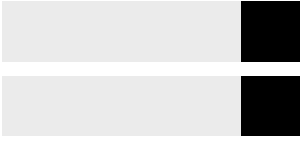
\includegraphics[width=.9\linewidth]{./img/palette-evidence.pdf}
\label{fig:Palette d'évidence}
\end{center}

\begin{center}
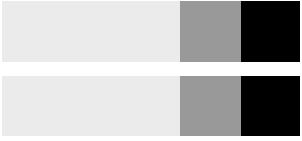
\includegraphics[width=.9\linewidth]{./img/palette-binaire.pdf}
\label{fig:Palette binaire}
\end{center}

\begin{center}

\includegraphics[width=.9\linewidth]{./img/palette-divergente.pdf}
\label{fig:Palette divergente}
\end{center}

\begin{center}
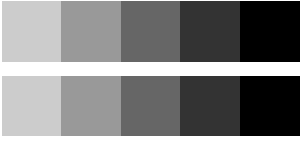
\includegraphics[width=.9\linewidth]{./img/palette-monochrome.pdf}
\label{fig:Palette monochrome}
\end{center}

\begin{center}
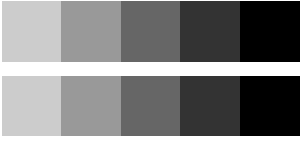
\includegraphics[width=.9\linewidth]{./img/palette-thermique.pdf}
\label{fig:Palette thermique}
\end{center}

\begin{center}
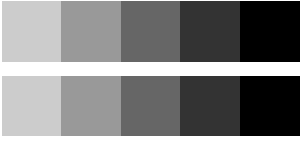
\includegraphics[width=.9\linewidth]{./img/palette-categorique.pdf}
\label{fig:Palette catégorique}
\end{center}
\section*{Tables}
\label{sec:orgfb1ddba}
Une table ou tableur permet d'exposer des données brutes organisées en lignes ou en colonnes. \autocite{mikeyiHowChooseRight2020}

Sauf mention contraire, les recommendations sur les tables sont issues du livre \og Show me the numbers\fg{} de Stephen Few.\autocite{stephenfewShowMeNumbers2012} L'auteur y rentre très en détails sur chaque point de paramétrage. Il y indique notamment les orientations en matière de construction de tableur lorsqu'il s'agit du choix premier d'affichage de données. Ce rapport s'intéresse à la conception de graphique. Dans ce cadre, les tableurs sont des éléments complémentaires pouvant être affichés par l'utilisateur pour explorer plus précisement les données préalablement affichées.

Des prescriptions spécifiques à la préparation de tableurs pour certains graphiques sont apportés le cas échéant dans la suite de ce rapport.
\subsection*{Composition}
\label{sec:org9b0d17d}
Il est recommendé de séparer les entrées avec un espace vide.
Lorsque les données sont présentées en colonnes, l'espace entre deux colonnes doit être plus grand qu'entre deux lignes,
Lorsque les données sont présentées en ligne, l'espace entre deux ligne doit être plus grand qu'entre deux colonnes,

Insérer une ligne vide toutes les 5 lignes pour faciliter le balayage visuel. \autocite{NFENISO9241-125ErgonomieLinteractionHommesysteme2017}

Utiliser une ligne horizontale pour séparer les entêtes de colonnes des données,

Utiliser une ligne horizontale pour séparer les catégories lorsque les données sont triées par catégories et, ne pas répéter le nom de la catégorie sur toutes les lignes. Les noms des catégories doivent être dans la première colonne, les sous-catégorie dans la seconde colonne, etc. S'il y a plusieurs subdivisions, les noms des catégories doivent être apposées sur la même ligne.

Il convient de rappeler le nom de la catégorie en cas de changement de page et de maintenir la structure du tableur sur toutes les catégories et de rappeler les titres des colones en cas de changement de page.
Les catégories doivent être ordonnées suivant un ordre logique (eg. chronologique, alphabetique, par classement, etc.)

Ne pas effectuer de rotation sur un tableur, son orientation doit respecter celle du texte du document.

Maintenir les aligmnements les titres avecc celui des données en colonnes.
\subsection*{Chiffres}
\label{sec:orgcaded3d}
Aligner les chiffres à droite.
Homogénéiser les décimales (généralement 2 ou 3 décimales suffisent suivant le contexte).
Indiquer les valeurs négatives avec le symbole \og moins\fg{} (-), ici la notion de valeur symbolique est importante. Certains choisissent d'identifier les valeurs négatives entre parenthèses, cependant il ne s'agit pas d'une représentation naturelle répendue pour une telle identification.
Séparer les digit d'un nombre par un espace tous les 3 charactères. Dans le cas de grands nombres, il convient de les arrondir à la précision utile (dixaine, centaine\ldots{}). Par défaut, la précision affichée doit correspondre à celle de la source d'information.
Si une valeur numérique réfère à une information de catégorie elle doit être traitée comme un texte.
\subsection*{Texte}
\label{sec:orgf65c7cf}
Aligner les textes à gauche.
Centrer les dates et utiliser une convention stricte d'écriture de ces données telles que \og YYYY-MM-DD\fg{}. \autocite{ISO8601-1DateHeureRepresentations2019} La composition de la date doit être indiqué à l'utilisateur. Le choix du format doit respecter le niveau de précision associée à la mesure. Implicitement, le choix d'un formatage de plus haut niveau que la précision de la mesure induit une agrégation des valeurs.
Centrer les données dont la largeur de charactère est fixe.
\subsection*{Sommaire et agrégats}
\label{sec:org3ab3e7e}
Utiliser une ligne verticale pour séparer les valeurs placées en colonne à droite de toutes les valeurs.
Utiliser une ligne horizontale si ces valeurs sont placées en une ligne en bas du tableau.
Si ces valeurs sont le message important de votre tableur, il convient de les affichés imédiatement à droite des colonnes de catégories ou immédiatement en dessous des entêtes de colonnes, suivant la nature du sommaire.

Les produits d'un calcul doivent être affichés dans la colonne imédiatement à droite de la colonne source de données.
\subsection*{Mise en évidence}
\label{sec:orgab80a4f}
Si des valeurs spécifiques doivent être mises en avant, il est possible d'utiliser l'une ou l'autre de ces solutions :
\begin{itemize}
\item mettre le texte en gras,
\item remplir la cellule d'une couleur.
\end{itemize}
Il est recommandé de limiter cette opération à un nombre réduit de valeur. Si cela n'est pas possible, il convient de sélectionner un autre mode de visualisation.
\section*{Méthode de sélection}
\label{sec:org27ce84c}

\section*{Graphiques}
\label{sec:org107d76d}
\subsection*{Arbre de mot}
\label{sec:org6b51685}
Représente les liens sémantiques. Utilisé pour classifier les réponses textuelles d'une enquête.(voir Paige Jarreau) Utilisé pour illustrer l'usage des mots dans un texte.(voir Martin Wattenberg \& Fernanda Viegas 2007) La taille des mots représente la fréquence de leurs usages. \autocite{jonathanschwabishQualitative2021}
\subsection*{Arc}
\label{sec:org8a1f521}
\sout{Hémicycle, souvent utilisé pour visualiser la composition d'un effectif.}
\subsection*{Arc temporel}
\label{sec:org11421a0}
Utilisé pour illustré les connexions des catégories à travers le temps. L'ordre des données influence la percéption de l'importance des connexions. \autocite{jonathanschwabishRelationship2021}

Peut être utilisé pour illustrer les distances entre deux points. Cet usage met bien en évidence l'augmentation des disances. \autocite{jonathanschwabishRelationship2021}
\subsection*{Bande de valeur}
\label{sec:org1a853cb}
Affiche les points de données d'une catégorie.\autocite{jonathanschwabishDistribution2021} Les valeurs peuvent être affichés par des lignes ou des cercles pleins mais les cercles sont à privilégier lorsqu'il est nécessaire de déagglomérer les données.

Il est possible d'utiliser de la transparence pour illustrer les zones de valeurs compactes. \autocite{jonathanschwabishDistribution2021} Utilisez la palette de couleurs divergentes \ref{fig:Palette divergente} pour mettre en évidence la répartition des valeurs mesurées et souligner la séparation de celles ci par rapport à un axe de référence.\autocite{jonathanschwabishDistribution2021}

Les points peuvent être légèrement décalés les uns des autres par un offset pour éviter le masquage de données par surimposition. Ce mode de représentation est appelé \og essaim d'abeille\fg{} (beeswarm). \autocite{jonathanschwabishDistribution2021}

Histopoint : Wilkinson dot plot (Leland Wilkinson) Affichage des bandes de valeurs pour chaque agrégat d'un histogramme.\autocite{jonathanschwabishDistribution2021}

Epis de blé : Wheat plot (SFew)
\subsection*{Barre divergente}
\label{sec:org675fc3e}
Affiche correctement un ensemble de valeur quantitative triées par catégories lorsque des valeurs négatives sont utilisées. \autocite{alansmithLexiqueVisuel} L'axe des absysse doit être égal à 0 et toutes les barres doivent être projetées depuis cet axe.
\subsection*{Barres divergentes empilées}
\label{sec:org8a2b9ed}
Utilisé pour illustrer les résultats d'enquêtes impliquant un sentiment. \autocite{alansmithLexiqueVisuel} Les barres doivent être calculées en pourcentage et alignées à 100\% comme pour une partie d'un ensemble. Les réponses sont affichées de façon ordonée et du plus négatif au plus positif. Il convient d'utiliser une palette de couleur divergente. Lors de la préparation d'une enquête impliquant des sentiment, il est conseiller de proposer un choix de valeur paires pour éviter les votes neutres sauf si la représentation de l'indiférence est une volontée de l'étude. De plus, \textbf{expliquer la limite de nombre de zones facile à visualiser} (max 6?)
\subsection*{Barre empilées}
\label{sec:org0c6bc4e}
Représente le total de chaque catégorie et la proportion de leurs composantes. Les composantes doivent être homogènes. Si les proportions sont plus importantes que les totaux, considérer d'utiliser l'affichage empilée à 100\%. \autocite{mikeyiHowChooseRight2020}

Seule la catégorie ayant sa base à 0 sera facile à comparer pour le lecteur car les autres ne partagent pas la même base.\autocite{jonathanschwabishComparingCategories2021} Il est préférable de tracer chaque diagramme de barre dans un grapgique distinct et des les disposer en \hyperref[sec:orge82e1e4]{Matrice de graphique}. \autocite{jonathanschwabishComparingCategories2021}
\subsection*{Barre jumelée}
\label{sec:org306a4de}
Permet d'afficher plusieurs séries. Devient plus difficile à lire avec plus de deux séries. \autocite{alansmithLexiqueVisuel}
Les barres d'une même catégories sont collées les unes aux autres pour souligner leurs appartenance à une même catégorie (ratio 1:0). Espacer les jeux de barres jumelées d'une largeur égale à une barre (ratio n:1).

Les barres sont colorées avec une palette de couleur de catégories. Les couleurs sont utilisées pour distinguées chaques barres dans une catégories, les couleurs doivent être homogènes pour chaque catégorie. Si les différentes valeurs affichées sont d'importances similaires, il convient d'utiliser une palette de couleurs à faibles contrastes. N'utiliser qu'une seule couleur par ensemble de données apparentées. \autocite{stephenfewComponentlevelGraphDesign2012}
\subsection*{Barre ordonnée}
\label{sec:org560419e}
Les catégories sont ordonnées par décroissance de leurs valeurs de quantité\autocite{jonathanschwabishComparingCategories2021} sauf si les catégories on un autre ordre logique (eg. temporel). Dans ce second cas, cet ordre doit être utilisé pour la construction du graphique. \autocite{wilkeVisualizingAmounts2019}

\textbf{Note: si catégories temporelles, utiliser un histogramme?}

Lorsqu'un ordre de classement est à afficher, l'utilisation d'un graphique horizontal est à privilégier. \autocite{andreaskrauseBestPracticesData2024}

\textbf{William Playfair (1786) pionnier de l'utilisation de ce type de graph ?}

Les barres doivent être affichées à l'horizontal s'il y a beaucoup de valeurs à afficher ou si les labels des catégories s'entrevêchent. \autocite{alansmithLexiqueVisuel,sosulskiGraphics2019,wilkeVisualizingAmounts2019,stephenfewComponentlevelGraphDesign2012,jonathanschwabishComparingCategories2021}

Il convient de maintenir l'affichage vertical du graphique si les catégories affichées sont des unitées temporelles. \autocite{stephenfewComponentlevelGraphDesign2012}

Ce graphique est plus lisible pour un nombre limité d'entrées. \autocite{mikeyiHowChooseRight2020}

L'espace entre deux barres est égal à la moitié de la largeur d'une barre (ratio 1:0.5). Les barres ont toutes la même largeur. \autocite{stephenfewComponentlevelGraphDesign2012}

Utiliser une couleur homogène à l'ensemble des barres. Une couleur de contraste peut être utilisée pour mettre en évidence certaines catégories.

Ne pas utiliser de motifs de remplissage. Les barres doivent être remplies par un solide coloré. \autocite{stephenfewComponentlevelGraphDesign2012}

Ne pas utiliser de bordures de barres. Ces dernières doivent naturellement contraster avec l'arrière plan.

Si de grands écarts de valeurs empêchent la bonne visualisation des écarts sur une partie du graphique, il est recommendé d'ajouter un second graphique en barre ordonnée n'affichant pas les catégories aux grandes valeurs. \autocite{jonathanschwabishComparingCategories2021}

Ne pas afficher de séparateurs au niveau des catégories, les barres remplissent elles même ce rôle, associées aux espaces entres elles. \autocite{jonathanschwabishComparingCategories2021}

Pour les petits graphiques statiques, il convient d'apposer directement un label à chaque barre contenant la valeur de celles-ci. Par cette action, il convient également de masquer l'axe des absysses. \autocite{jonathanschwabishComparingCategories2021}

Pour les graphiques dynamiques, interractifs ou de grande largeur, il convient d'afficher des lignes d'aide à la lecture en projection des repères de l'axe des valeurs. Ces lignes doivent être faiblement contrastées et être tracées en arrière plan des barres. \autocite{jonathanschwabishComparingCategories2021}

Ne pas segmenter les barres. \autocite{jonathanschwabishComparingCategories2021}

Ne pas ajouter d'iconographie aux barres. \autocite{tranDiscoveringAccessibleData2024}
\subsection*{Bulle proportionnelle ordonnée}
\label{sec:orgc864574}
Utilisé pour illustrer les grandes variations de quantité pour différentes catégories et lorsque la distinction des nuances n'est pas primordiale. Les bulles doivent être dimensionnés par leurs surface pour éviter d'éxagérer les différences. \autocite{jonathanschwabishComparingCategories2021} Ce type de graphique utilise un double encodage de la quantité : la position et la taille. \autocite{wilkeVisualizingAssociationsTwo2019} Bien que ce type de représentation soit considéré comme engageant, il convient d'utiliser un graphique en barre ordonnée à la place lorsque l'évaluation des différences entre catégories est importante. \autocite{jonathanschwabishComparingCategories2021}
\subsection*{Boite à moustache}
\label{sec:org94a591b}
Résume les distributions multiples en montrant la médiane et l'étendue des données. \autocite{alansmithLexiqueVisuel}

Ce graphique est plus efficace lorsqu'il y a de nombreuses mesures pour une entrée et que leur distribution doit être représentée (eg : mesure médiane, basse, haute, incertitude\ldots{}). \autocite{mikeyiHowChooseRight2020}

Les lignes s'étendant au dessus et en dessous sont appelées les moustaches. \autocite{wilkeVisualizingManyDistributions2019}

\textbf{Voir trx de son inventeur : John W. Tukey}

Il est possible d'afficher la position d'un point précis du jeu de donnée sous-jacent. (couleurs mise en évidence ?)

Les boites à moustaches suivent les dispositions graphiques des barres ordonnées. \autocite{stephenfewComponentlevelGraphDesign2012}
\subsection*{Bosses}
\label{sec:orgf04b2b2}
Affiche l'évolution d'un classement entre différents jalons. \autocite{mikeyiHowChooseRight2020,alansmithLexiqueVisuel}  Ce graphique n'affiche pas les valeurs sous-jacente mais uniquement le positionnement de la catégorie dans le classement. \autocite{jonathanschwabishTime2021} Si la valeur source est également à représenter, ce graphique peut se transformer en graphique en ruban, combinant les disposition du graphique en bosse avec celles du graphique de Sankey. \autocite{jonathanschwabishTime2021}
\subsection*{Camembert}
\label{sec:org16fc732}
Diagramme standard, difficile à lire. \autocite{alansmithLexiqueVisuel}
Limiter à 5 (4?) entrées maximum \autocite{mikeyiHowChooseRight2020}

Ce graphique doit être limité à l'illustration d'un état donnée. Il est important de garder à l'esprit que ce graphique ne donne qu'une représentation et n'est pas adapté à l'affichage de valeurs précises. \autocite{jonathanschwabishParttowhole2021}

Le camembert permet d'accentuer l'appartenance d'une partie individuelle à un ensemble homogène et complet. Il illustre parfaitement des fractions simples.\autocite{wilkeDirectoryVisualizations2019} Les quantités n'ont pas leurs place dans un camembert, ce sont les fractions (taux, pourcentages) qui y sont illustrés. Ainsi, l'ensemble des valeurs constituante sont strictement égale à 100\% du total.\autocite{wilkeVisualizingAmounts2019} Il représente plus efficacement les parts dont les angles sont familiers aux lecteurs soit respectivement 90°, 180° et 240° pour les taux 25\%, 50\% et 75\%.

Ce graphine n'est pas adapté à ces cas de figure :
\begin{itemize}
\item les parts sont de tailles similaires,\autocite{sosulskiGraphics2019}
\item Il y a beaucoup de catégories à afficher pour atteindre l'objectif du message,
\item il y a une comparaison entre deux graphiques à réaliser,\autocite{jonathanschwabishParttowhole2021}
\item il y a un changement entre plusieurs états.\autocite{wilkeDirectoryVisualizations2019}
\end{itemize}

Il convient de :
\begin{itemize}
\item Arranger les parts par orgre de valeur croissant en commençant à '12h'. \autocite{jonathanschwabishParttowhole2021}
\item Utiliser un espace vide entre chaque part pour les faire resortir, \autocite{sosulskiGraphics2019}
\item Utiliser une palette de couleur de mise en évidence pour faire ressortir une seule part ou,
\item Utiliser une palette de couleur pour faire resortir deux parts,
\item Apposer les labels directement sur les parts au moyen d'étiquette. \autocite{sosulskiGraphics2019}
\end{itemize}

Les parties n'étant pas mises en avant peuvent être agrégée en une catégories \og autres\fg{}. Leurs informations ne servant pas à appuyer le message du graphique. \autocite{jonathanschwabishParttowhole2021}

Dans le cas ou une seule partie de l'ensemble est mise en avant, il est à considérer l'utilisation d'un \hyperref[sec:org200724a]{Marqueur}. Le camembert n'apportant aucune information particulière à votre propos.

Il n'est pas encore clairement établis si la comparaison des valeurs est réalisé par la perception des angles ou par la perception des longueurs d'arcs des différentes parties.\autocite{jonathanschwabishParttowhole2021}

Ce diagramme possède un avantage majeur au regard des autres modes de représentation des parties d'un ensemble, il est très populaire et ainsi accessible à usager. \autocite{jonathanschwabishParttowhole2021} Il est également reconnu que les formes circulaires attirent l'intéret des utilisateurs.\autocite{jonathanschwabishParttowhole2021}
\subsection*{Carte de fréquentation}
\label{sec:orgd8ef381}
Excellente visualisation pour suivre la fréquence d'une activité. Favorise la quantité à la qualité (exemple : github). \autocite{alansmithLexiqueVisuel}
\subsection*{Cascade}
\label{sec:org3f67768}
Affiche les gains et pertes entres deux états d'un système. \autocite{jonathanschwabishComparingCategories2021} Utilisé principalement pour les analyses financières. \autocite{alansmithLexiqueVisuel}
\subsection*{Chandelier}
\label{sec:orgf44f7e0}
Affiche des bilans quotidiens (eg. ouverture, fermeture, point haut, point bas). \autocite{alansmithLexiqueVisuel}
La couleur est utilisée pour représenter la direction de l'évolution de la valeur (augmente, descend).

Illustre les évolutions d'un stock sur une temporalité donnée. La ligne indique l'état le plus haut et l'état le plus bas de la journée. La barre indique l'état de l'ouverture et de la cloture de la période. \autocite{jonathanschwabishDistribution2021} Il convient d'utiliser une palette de couleur binaire pour contraster les périodes aux soldes positifs des périodes aux soldes négatifs.
\subsection*{Chronologie circulaire}
\label{sec:org7c28ca3}
Pour l'affichage des valeurs discrètes de taille variable à travers de multiples catégories. \autocite{alansmithLexiqueVisuel}
\subsection*{Chronologie verticale}
\label{sec:org6f2c054}
Affiche le temps sur l'axe Y. Particulièrement adapté à l'affichage sur mobile. \autocite{alansmithLexiqueVisuel}
\subsection*{Colonne vertébrale}
\label{sec:org905e10a}
Utilisé pour afficher la quantité de réponses négatives et positives à une question. Le spine divise une valeure quantitative unique en deux ccomposants distinct contrasté par un déterminent binaire. \autocite{alansmithLexiqueVisuel} Utilisé pour afficher la quantité de réponses négatives et positives à une question.
\subsection*{Coordonnées parallèles}
\label{sec:orgc82d73c}
Montre en simultané la valeur et la relation de catégories hétérogènes pour plusieurs systèmes. \autocite{jonathanschwabishRelationship2021} Permet de valoriser la valeur. \autocite{alansmithLexiqueVisuel}

Pratique pour observer les schémas et relations entre les systèmes. \autocite{mikeyiHowChooseRight2020} Ce graphique est plus efficace pour explorer des jeux de données que pour les présenter à un audimat. \autocite{sosulskiGraphics2019}

Chaque axes de catégories peut avoir sa propre échelle. Cela représente mieux les valeurs de chaque catégorie mais cela implique également de bien labeliser les axes pour distinguer leurs échelles. \autocite{jonathanschwabishRelationship2021}

Afficher un grand nombre de jeux de données sur un même graphe risque de le rendre illisible. \autocite{jonathanschwabishRelationship2021} Dans ce cas il convient d'utiliser une palette de couleur de mise en évidence et de selectionner un ou deux jeux de données à mettre en avant.

Lors de l'exploration d'un jeu de donnée à travers une interface informatique, il convient de mettre en avant la ligne pointée par l'utilisateur et de labeliser chaque points de catégorie avec la valeur associé. \autocite{sosulskiGraphics2019}
\subsection*{Corde}
\label{sec:org3f1373d}
Illustre les flux bidirectionnels et le gagnant net dans une matrice. \autocite{alansmithLexiqueVisuel}

Dans la mesure du possible, il convient de flécher le sens du flux.

Ce diagramme incite les utilisateurs à l'explorer plus en détail. \autocite{jonathanschwabishRelationship2021}
\subsection*{Courbe cumulative}
\label{sec:orgb03b8e4}
Utilisé pour représenter une distribution inégale. L'axe des ordonnées est toujours la fréquence cumulative et l'axe des absisses est toujours une mesure. \autocite{alansmithLexiqueVisuel}
\subsection*{Courbe de densité}
\label{sec:org4bcd8df}
La densité représente la probabilité de distribution des variables. \autocite{sosulskiGraphics2019} Pertinent lorsque le nombre de données est très grand, autrement il convient d'utiliser un histogramme. \autocite{wilkeVisualizingManyDistributions2019} En cas d'affichage de plusieurs courbe, utiliser  des remplissages transparents pour faciliter la distinctions. L'air de la courbe est usuellement égal à 1 et de ce fait, l'échelle de l'axe des ordonnées dépend de l'axe des absisses. \autocite{wilkeVisualizingManyDistributions2019}
\subsection*{Donut}
\label{sec:org6a1c6bc}
Dans un graphique en donut, les valeurs sont à comparer en fonction des longueurs d'arcs.

Comme le diagramme circulaire, le centre peut être utilisé pour afficher un total ou encore une icone. \autocite{alansmithLexiqueVisuel}

Il est, autrement, en tout point similaire aux \hyperref[sec:org16fc732]{Camembert}
\subsection*{Etats parallèles}
\label{sec:org16328e5}
Montre les changements sur un flux entre un état et au moins un autre. Adapté au traçage d'un processus complexe. \autocite{alansmithLexiqueVisuel}
Cette représentation découpe un ensemble en quantité individuelles de plusieurs catégories. Les bandes sont tracées entre chaque catégories pour représenter leurs relations. La largeur des bandes indiquent la proportion des catégories correllées les unes aux autres. \autocite{wilkeVisualizingNestedProportions2019}
A utiliser à la place des mosaiques et treemaps lorsqu'il y a plus de deux variables de regroupement des données. \autocite{wilkeDirectoryVisualizations2019}
\subsection*{Eventail}
\label{sec:org5e2d473}
Utilisé pour montrer l'incertitude des projections futures. \autocite{alansmithLexiqueVisuel}
\subsection*{Frise de Priestley}
\label{sec:orgd83fe36}
Parfait lorsque la date et la durée sont des éléments clés dans l'histoire de la donnée. \autocite{alansmithLexiqueVisuel}
\subsection*{Haltères}
\label{sec:org8e8c130}
Utilisé pour comparer un minimum et un maximum de plusieurs catégories. \autocite{alansmithLexiqueVisuel} La relation entre le maximum et le minimum d'une catégorie est représenté par la barre reliant les deux valeurs. \autocite{mikeyiHowChooseRight2020}

Peut être utilisé pour illustrer le changement d'une valeur entre deux état données. Dans ce cas, il convient de flécher le sens du changement de l'état antérieur vers l'état final.

Dans ces deux cas de figures, les catégories doivent êtres ordonnées de la plus grande valeur à la plus petite.

Les haltères sont toujours affichés à l'horizontal.
\subsection*{Histogramme}
\label{sec:orgfcf5166}
Utilisé pour afficher la fréquence d'une variable simple regroupée en intervale de fréquence (agrégat).\autocite{sosulskiGraphics2019} Il affiche ainsi une distribution statistique de donnée. Il n'y a pas d'espace entre deux barres (ratio 1:0) ce qui permet de favoriser la forme de la distribution. \autocite{alansmithLexiqueVisuel}

La nature du graphique (barre) implique un calcul d'agrégat pour chaque barre. \autocite{wilkeVisualizingDistributionsHistograms2019} La largeur de l'agrégat est à évaluer par le concepteur au regard du niveau de détail souhaité.\autocite{wilkeVisualizingDistributionsHistograms2019}

L'histogramme n'est pas adapté aux cas suivant :
\begin{itemize}
\item l'affichage de l'ensemble des valeurs, pour cela il convient d'utiliser une \hyperref[sec:org4bcd8df]{Courbe de densité}. \autocite{wilkeVisualizingDistributionsHistograms2019}
\item s'il y a peu de valeurs dans le jeu de données, \autocite{weissgerberBarLineGraphs2015} préférez l'utilisation d'une \hyperref[sec:org1a853cb]{Bande de valeur}.
\item l'affichage de plusieurs distributions,\autocite{wilkeVisualizingDistributionsHistograms2019} utilisez une décomposition en \hyperref[sec:orge82e1e4]{Matrice de graphique}.
\end{itemize}

L'utilisation d'un histogramme permet d'identifier des schémas de distributions tels que : \autocite{jonathanschwabishDistribution2021}
\begin{itemize}
\item \textbf{Incliné à gauche :} les données sont majoritairement sur la gauche du graphique
\item \textbf{Incliné à droite :} les données sont majoritairement sur la droite du graphique
\item \textbf{Bimodale :} lorsque deux pics de valeurs sont constatables
\item \textbf{Multimodale :} lorsque plus de deux pics de valeurs sont constatables
\item \textbf{Symétrique :} lorsqu'il y a un nombre approximativement égal de valeurs de chaque coté d'une valeur centrale
\item \textbf{Uniforme :} lorsque toutes les valeurs sont distribuées de façon globalement homogène
\end{itemize}
\subsection*{Horizon}
\label{sec:orgac5f79b}
Permet de vérifier un équilibre entre deux borne par rapport à une base. \autocite{alansmithLexiqueVisuel}  Utilisé pour suivre l'évolution d'une variable dans le temps et devant respecter un écart-type (eg. tension à 230V +/- 5\%). L'information la plus importante est le dépassement de l'écart-type. Pour correctement mettre en évidence ces phénomènes, il est recommendé d'utiliser une palette de couleur de
\subsection*{Jauge}
\label{sec:org94e9b30}
Représentation métaphorique la vitesse d'un système.
\subsection*{Ligne}
\label{sec:org966d7db}
Inventé par Playfair en 1786 \autocite{sosulskiBecomingVisual2019}
Représentation graphique standard et famillière pour la représentation des séries temporelles. \autocite[,@Schwabish2021p86]{alansmithLexiqueVisuel}

Les lignes relient chaque point de mesure. Pour de grands jeux de données, il convient d'utiliser une ligne lissée sur l'ensemble du graphique plutot qu'une ligne brisée par chaque point de donnée. \autocite{wilkeDirectoryVisualizations2019}

La base des ordonnées doit être égale ou inférieure à la plus faible valeur affichée. \autocite{Wong2010}

Il n'existe pas de rêgle stricte quand à la limite de séries affichables sur un graphique.\autocite{jonathanschwabishTime2021} Il convient de s'intéresser à la perception du lecteur recherché par le concepteur pour arbitrer les choix : \autocite{jonathanschwabishTime2021}
\begin{itemize}
\item En cas d'impression, limiter le nombre de lignes simultanées à 4 au maximum, \autocite{Wong2010}
\item Si l'interraction est possible avec le graphique, il est possible de tracer toutes les lignes dans un même graphique à condition d'utiliser un système de mise en évidence,\autocite{jonathanschwabishTime2021}
\item Ces cas échouant, séparez les lignes et tracez une \hyperref[sec:orge82e1e4]{Matrice de graphique}.
\end{itemize}

Ne pas utiliser ce graphique pour essayer d'illustrer une différence entre deux courbes. \autocite{jonathanschwabishTime2021}

Les axes doivent être labelisé (obligatoirement le titre de la série, optionnellement la valeur finale) directement en fin de ligne, à droite du graphique. \autocite{andreaskrauseBestPracticesData2024,sosulskiGraphics2019}

Il est possible de mettre en évidence un point spécifique en utilisant un symbole (de préférence un cercle plein) et en y apposant une étiquette affichant \(f(x)=y\).

La distinction des séries est plus efficace en utilisant des teintes différentes. Dans ce cas, il convient également d'utiliser des tons différents pour assurer le maintiens des distinctions si le graphique est imprimé en nuance de gris. \autocite{stephenfewComponentlevelGraphDesign2012}
Il convient également de n'utiliser que des lignes continues pour les tracés. \autocite{stephenfewComponentlevelGraphDesign2012}
L'utilisation de symboles comme éléments différenciants entre les séries n'est pas pertinent. \autocite{stephenfewComponentlevelGraphDesign2012}
\subsection*{Ligne de crête}
\label{sec:org025bc04}
Ce graphique représente des courbes de densité séparées par un offset et est utilisé pour comparer la distribution d'une vrariable entre des catégories. \autocite{wilkeVisualizingManyDistributions2019} Parfait lorsque les schémas de distributions sont bien distincts entre les groupes. \autocite{mikeyiHowChooseRight2020} Cela évite que les courbes de densités des catégories s'entrevêchent.\autocite{jonathanschwabishDistribution2021}

Ce graphique se met très bien à l'échelle de grands jeux de données. \autocite{wilkeVisualizingManyDistributions2019}

Il est adapté à :
\begin{itemize}
\item la comparaison des changements de distributions à travers le temps \autocite{wilkeDirectoryVisualizations2019} associé à un gradiant de couleur pour diriger le regard vers la distribution la plus récente, \autocite{jonathanschwabishDistribution2021}
\item la comparaison des évolutions de deux tendances à travers le temps. \autocite{wilkeVisualizingManyDistributions2019} associé à une palette de couleur binaire.
\end{itemize}

L'axe des absysses affiche la valeur de réponse et l'axe des ordonnées affiche les catégories. \autocite{wilkeVisualizingManyDistributions2019}

Il convient de classer les catégories suivant un ordre logique. \autocite{jonathanschwabishDistribution2021} Voir (insérer renvois ici vers l'explication de la logique de classement de catégories)

Il est possible d'afficher les barres d'erreurs dans les lignes de crêtes. Ce mode de représentation s'appel un \og demi-oeil\fg{}. \autocite{wilkeVisualizingUncertainty2019}

Il est possible d'afficher les nuages de points dont l'estimation de la courbe de densité est issue. Ceux-ci sont affichés en dessous des courbes de densité. Cette forme de représentation est appelé \og Nuage de pluie\fg{}. (ref: Micah Allan ou Schwabish2021p212) Cette représentation offre à la fois une représentation générique et une visualisation précise des données. \autocite{jonathanschwabishDistribution2021} Bien que cette représentation soit très efficace, elle n'est pas très répendue. \autocite{jonathanschwabishDistribution2021} Il faut être vigilent à bien expliquer son fonctionnement lors de son utilisation dans un rapport. Dans le cas d'un nuage de pluie, il faut faire attention à ce que les points de données n'entre pas en surimposition avec les courbes de densitées tracées en dessous.
\subsection*{Lollipop}
\label{sec:org67e04b1}
Utilisé pour afficher la position dans une liste ordonnée lorsque l'affichage de la valeur est moins important que la position. \autocite{alansmithLexiqueVisuel} Egalement très efficace comparé aux barres hordonnées lorsqu'il y a un grand nombre de catégorie dans le classement. \autocite{mikeyiHowChooseRight2020}  Si une ligne connecte le point de la valeur à laxe des ordonnées, l'axe des absisse doit commencer à 0, autrement cela n'est pas obligatoire.
\subsection*{Marqueur}
\label{sec:org200724a}
Affiche une valeur simple, plus pertinent lorsqu'associé à une tendance sur une période donnée. \autocite{mikeyiHowChooseRight2020}
\subsection*{Marimeko}
\label{sec:org7254e9e}
Visualisation de la taille et des proportions d'un ensemble homogène de données. \autocite{alansmithLexiqueVisuel}
Exemple : répartition des parts de marché de 3 entreprises sur un axe et taux dans 3 catégories de marché pour chacune

La couleur peut être utilisée pour mettre en évidence une valeur. \autocite{jonathanschwabishComparingCategories2021} Attention au biais de correlation lorsque ce graphique est utilisé pour représenter plusieurs variables. \autocite{jonathanschwabishComparingCategories2021}
\subsection*{Matrice de bulle}
\label{sec:orgddace64}
Ce graphique est une version aggrégée du nuage de bulle et le la matrice de température.

Il simplifie la visualisation des relations entre un couple de variable. A réserver pour un usage d'exploration de donées. \autocite{sosulskiGraphics2019} La taille des bules représente la force de la corrélation. Cette force est la représentation du coefficient de Pearson. \autocite{jonathanschwabishRelationship2021}

La couleur peut être utilisée pour distinguer les catégories (à vérifier). Elle peut être également utilisée comme double encodage de la correlation (à vérifier).

Le tableur associée est une matrice de correlation organisant les valeurs de coefficient de Pearson.
\subsection*{Matrice de graphique}
\label{sec:orge82e1e4}
Origine
Est utilisé pour comparer de multiples graphiques homogènes organisées en matrices. Chaque entité affiche le graphique d'une catégorie. Les graphiques sont tous à la même échelle. \autocite{sosulskiGraphics2019}

Conseils : Limitez les détails dans chacun des graphique. \autocite{sosulskiGraphics2019} Regroupez les axes pour n'afficher qu'un seul axe Y par ligne et un seul axe X par colonne.
\subsection*{Matrice de température}
\label{sec:org13246bb}
Représentation graphique d'une table de valeur homogène. \autocite{sosulskiGraphics2019}
Intéressante pour afficher une tendance lorsqu'un très grand nombre d'information est impliqué.

En utilisant une palette de couleur séquentielle, un lecteur aura tendance à considérer une couleur sombre comme une valeur haute. En utilisant une palette de couleur divergente (eg. basée sur la température de la couleur), ce phénomène s'estompe.

L'organisation des catégories changeant la forme de la matrice de température, il convient de retenir une organisation par valeur croissante ou décroissante à une colonne donnée. Il convient de signaler cette configuration au lecteur. \autocite{wilkeVisualizingAmounts2019}
\subsection*{Mini-graphe}
\label{sec:orga81717d}
Affiche la tendance d'évolution d'une variable ou d'une catégorie. Est généralement intégré dans un tableur. Un mini-graphe ne possède pas d'axes ni d'autres détails et est composé uniquement d'une courbe et d'un point indiquant la dernière valeur du jeu de donnée. \autocite{sosulskiGraphics2019} Cette représentation est très macroscopique et vise à succiter un sentiment plutot que d'exposer une valeur précise. \autocite{jonathanschwabishDistribution2021}

Un mini-graphe ne possède pas d'axes ni d'autres détails.
\subsection*{Nuage de bulle}
\label{sec:org30df561}
Il s'agit d'un nuage de point dont la taille des bules est utilisé pour représenter une troisieme valeur quantitative. \autocite{alansmithLexiqueVisuel}
\subsection*{Nuage de mots}
\label{sec:org4671765}
Affiche des nuages de mots organisés en groupes sémantiques. La taille des mots indique leur fréquence d'utilisation dans le corpus étudié. La couleur des groupes peut représenter un choix de données qualitative (catégorisation). \autocite{sosulskiGraphics2019} Cette visualisation est une méthode d'exploration de texte utile pour réaliser une synthèse macroscopique.
Il convient de filtrer les mots vides dit \og stopwords\fg{} pour nettoyer la composition des nuages. \autocite{jonathanschwabishQualitative2021} Des listes de mots vides peuvent être trouvées à l'adresse \url{https://github.com/stopwords-iso/}.
\subsection*{Nuage de point}
\label{sec:orgf0402a2}

\includegraphics[width=1.2cm]{./img/icon-scatterplot.pdf}
Représente la relation entres deux variables continues. \autocite{alansmithLexiqueVisuel}
La couleur est utilisée pour distinguer les catégories.

Si des milliers de point de données sont à afficher, il est préférable d'utiliser soit :
\begin{itemize}
\item des cercles ouverts
\item des petits cercles
\item des cercles avec une transparence
Cela permet de limiter le masquage des points de données par surimposition. \autocite{andreaskrauseBestPracticesData2024}
\end{itemize}
\subsection*{Nuage de point connecté}
\label{sec:org7b4f0bb}
Montre l'évolution des données pour deux variables pertinentes si le modèle de progression est clair. \autocite{alansmithLexiqueVisuel}

Pour souligner la direction de l'évolution entre deux points il est possible de :
\begin{itemize}
\item Flécher la direction de l'évolution entre deux points si les points sont bien espacés et qu'un seul jeu de donnée est affiché, \autocite{jonathanschwabishComparingCategories2021}
\item Utiliser un gradiant de couleur du plus clair vers le plus foncé.
\end{itemize}

Ce graphique sers à synthétiser des variations de valeurs, il est préférable de l'utiliser pour afficher des jeux de données dont la variation n'est pas mesurée régulièrement pour éviter d'avoir trop de points à relier et donc d'éviter de créer un graphique trop encombré. \autocite{jonathanschwabishComparingCategories2021}
\subsection*{Pareto}
\label{sec:org07b8738}
Ce type de graphique montre la relation entre les valeurs quantitatives de catégories organisées en colonne ordonnée et la valeur cumulée affichée en ligne brisée. Le premier point de la ligne vérifiant \(\tau\geq80\%Total\) est affichée. La zone précédent ce point est mise en évidence.
Est utilisé pour illustrer les éléments important dans un système qualité.
\subsection*{Pente}
\label{sec:org77e9b8f}
Affiche la variation des valeurs ou ratios des catégories entre deux états donnés. \autocite{alansmithLexiqueVisuel}
\subsection*{Pictographe}
\label{sec:org7b843d8}
Utilisation hautement contextuelle limiter strictement à l'affichage d'entiers naturels. \autocite{alansmithLexiqueVisuel}
Les pictographes peuvent augmenter significativement la précision d'acquisition d'un écart de ratio ainsi que la rapidité de la visualisation d'un minimum ou d'un maximum entre des catégories. \autocite{tranDiscoveringAccessibleData2024} A la manière des symboles groupées, si la transmission de valeurs précise est importante, il convient d'utiliser un graphique en barre ordonnée à la place. \autocite{tranDiscoveringAccessibleData2024}
\subsection*{Polygone de fréquence}
\label{sec:org95358ad}
Utilisé pour afficher simultanément plusieurs distributions de données. Fonctionne comme un histogramme. Chaque agrégat est représenté par un point et ils sont reliés entres eux par un segment droit. Pour faciliter la lécture, il convient de limiter le nombre de distributions affichées à 4 \autocite{alansmithLexiqueVisuel} ce qui correspondant notamment au nombre de symboles aisément discriminables.
\subsection*{Quadrillage}
\label{sec:org894035c}
Adapté à l'affichage des informations en pourcentages. Fonctionne mieux avec des entiers naturels. \autocite{alansmithLexiqueVisuel} Généralement en grille de 10 x 10 carrés (pour un total de 100). Chaque carré représente 1\% d'un tout. Les carrés sont colorés sur la base de la taille d'une catégorie dans un groupe. \autocite{mikeyiHowChooseRight2020}
\subsection*{Radar}
\label{sec:org247efca}
Représentation compacte de la valeur de variables hétérogènes pour un seul système. \autocite{alansmithLexiqueVisuel} Les radards sont utilisés pour identifier les variables ayant des valeurs similaires et les exceptions. \autocite{sosulskiGraphics2019}

La représentation des valeurs se fait à travers la forme globale du polygonne. Il convient de coloriser l'interrieur de celui-ci pour bien faire ressortir sa forme. \autocite{jonathanschwabishRelationship2021}

Utiliser une disposition en small-multiples plutot que de surimposer plusieurs polygones de valeurs. \autocite{jonathanschwabishRelationship2021}

La représentation des variables est fortement correlé à la forme du polygone plutot qu'aux valeurs des sommets. \autocite{sosulskiGraphics2019} De ce fait, pour améliorer la forme du polygonne et offrir une représentation avec le moins de distortions possibles, il convient d'homogénéiser les échelles des axes.
\subsection*{Réseau}
\label{sec:orgd3ba3ee}
Utilisé pour montrer la force et l'interconnectivité des relations de types différents. \autocite{alansmithLexiqueVisuel} La position des nœuds n’a pas de fonction logique. Elle vise à rendre le diagramme le plus lisible possible. \autocite{mikeyiHowChooseRight2020}
\subsection*{Ruisseau}
\label{sec:org1c46c41}
Vérifier la méthafore liée au nom

A privilégier lorsque la visualisation des changements en proportions au fil du temps est plus importante que les valeurs individuelles. \autocite{alansmithLexiqueVisuel}
\subsection*{Sankey}
\label{sec:org227198c}
Créé par : Matthew Henry Phineas Riall Sankey (1898)
L'épaisseur représente la part d'un évènement. Chaque flèche représente l'entrée ou la sortie d'élément sur le système étudié. \autocite{mikeyiHowChooseRight2020}

Les changements sont liés à une évolution temporelle et à l'association de catégories. La force de ce graphique est qu'aucun de ces deux aspect ne pévaut sur l'autre. \autocite{jonathanschwabishComparingCategories2021}

Très utile pour représenter les flux entre des catégories ou entre des états. \autocite{jonathanschwabishComparingCategories2021}

Il convient néanmoins de limiter le nombre de catégorie  affiché pour maintenir un bon niveau de lisibilité. \autocite{jonathanschwabishComparingCategories2021}
\subsection*{Sismographe}
\label{sec:org64009ee}
Pour montrer des séries à grandes variation dans les données. \autocite{alansmithLexiqueVisuel}
\subsection*{Symbole groupé}
\label{sec:org210b124}
Utile lorsqu'il est utile de compter ou de mettre en évidence des éléments individuels organisés en barre ou en colonne. \autocite{alansmithLexiqueVisuel} Cependant, ce type de graphique n'est pas efficace dans cette action car il incite le lecteur à compter chaque point, ce qui peut s'avérer décourageant. \autocite{stephenfewSillyGraphsThat2012} Un certain usage peut être imaginé à des fins décoratives visant à illustrer un élément déjà explicité dans un texte. Un graphique en barre ordonné est à privilégier aux symboles groupés.
\subsection*{Tiret}
\label{sec:org888b315}
Présentation d'une valeur mesurée ou calculée au regard d'une valeur cible. \autocite{alansmithLexiqueVisuel} Pertinent lors de la réalisation d'un benchmark. \autocite{mikeyiHowChooseRight2020}
\subsection*{Tunnel}
\label{sec:org5606f37}
Utilisé pour suivre l'engagement d'une population (taille) à chaque étape d'un processus (barre). \autocite{mikeyiHowChooseRight2020}
\subsection*{Treemap}
\label{sec:org95be1c6}
Utilisé pour les relations hiérarchiques d'une partie vers l'ensemble. Difficile à lire s'il y a trop d'éléments affichés. \autocite{alansmithLexiqueVisuel}
Le découpage des boites n'a pas besoin d'être ordonné, il peut y avoir plus de 2 niveaux de hiérarchie. \autocite{mikeyiHowChooseRight2020}
\subsection*{Valeur lettrée}
\label{sec:org43f8f41}
Représente chaque découpage statistique (\(x\sigma\)) par une boite distincte. Convient en remplacement des boites à moustache lorsqu'il y a un très grand nombre de données disponibles. Permet de faire des estimations fiables. \autocite{hofmannLettervaluePlotsBoxplots2017,mikeyiHowChooseRight2020}
\subsection*{Violon}
\label{sec:orgaf69444}
Représente fidèlement les distributions d'un très grand nombre de données. \autocite{alansmithLexiqueVisuel} Utilisé pour faire des comparaisons entre des catégories. \autocite{mikeyiHowChooseRight2020}  Très pertinent pour représenter les distributions bimodales. \autocite{wilkeVisualizingManyDistributions2019} Le tracé du demi-violon est identique au tracé d'une courbe de densité. Celui-ci commence à la valeur la plus petite et termine à la valeur la plus grande.
\subsection*{Voronoi}
\label{sec:org9fa0263}
Semblable à un diagramme de bulle mais transformées en zones dont l'ensemble des points de chacune est plus proche du centre de sa zone que de tout autre centroïde. \autocite{alansmithLexiqueVisuel}

Il est très pertinent pour illustrer les parties d'un ensemble lorsque de nombreuses sous-catégories sont à afficher. \autocite{jonathanschwabishParttowhole2021} En ce sens, il est préféré aux camenberts.
\section*{Etudes futures}
\label{sec:org31eb738}
Des études complémentaires pourraient être menées sur les sujets suivants :
\begin{itemize}
\item La conception de librairies de graphiques accessibles et fonctionnant aussi bien dans un usage web que dans les PDF,
\end{itemize}
\section*{Evolution}
\label{sec:org4f839e3}
\begin{center}
\begin{tabular}{rl}
Date & Changements\\
\hline
2025-02-10 & Rédaction du document\\
\end{tabular}
\end{center}
\section*{Références}
\label{sec:org9ca36c5}
\printbibliography[heading=none]
\end{document}
